
\begin{Ejemplo}{\textbf{Tubo de deriva}}

En est ejemplo vamos a considerar un tubo de deriva con un diámetro de 15 mm y un diámetro del hilo (cable) de 50 $\mu m$, similar a los tubos de derivas de muones del ATLAS (también con un diámetro pequeño) llamados sMDTs. Primero importamos los módulos: \\

\begin{lstlisting}[language=C++,style=c++]
#include "Garfield/MediumMagboltz.hh"
#include "Garfield/ViewMedium.hh"
\end{lstlisting}

\vspace*{1em}


Lo primero que tenemos que hacer es preparar la \textbf{tabla de gases}, es decir, la tabla que contiene los parámetros de transporte (velocidad de deriva, coeficientes de difusión, coeficiente de Townsend, coeficiente de captura) como funciones del campo eléctrico $\Encal$ (y en general, del campo magnético $\Bn$ y el ángulo entre $\Encal$ y $\Bn$) para un gas a una temperatura y presión determinadas. En este ejemplo usaremos un gaz mezcla, a 3 atm y temperatura ambiente: \\

\begin{lstlisting}[language=C++,style=c++]
MediumMagboltz gas("ar", 93., "co2", 7);
// Set temperature [K] and preasure [Torr]
gas.SetPressure(3*760.);
gas.SetTemperature(293.15);
\end{lstlisting}

\vspace*{1em}

También debemos especificar el número de puntos de la malla campo eléctrico que vamos a usar en la tabla y el rango que va a ser cubierto. Usamos 20 puntos entre 100 V/cm a 100 kV/cm con un espaciado logaritmico:   \\

\begin{lstlisting}[language=C++,style=c++]
gas.SetFieldGrid(100.,100.e3,20,true);
\end{lstlisting}

\vspace*{1em}
    
Ahora ejecutamos Magboltz para generar una tabla del gas para esta malla de campo eléctrico. Como un parámetro de entrada tenemos que especificar \textit{el número de colisiones} (en múltiplos de $10^7$) sobre el electrón cuya traza dibuja Magboltz: \\

\begin{lstlisting}[language=C++,style=c++]
const int ncolll=10;
\end{lstlisting} 

Aunque tarde un rato, una vez este acabado podemos guardar los parámetros:  \\

\begin{lstlisting}[language=C++,style=c++]
gas.WriteGasFile("ar_93_co2_7.gas");
\end{lstlisting} 

\vspace*{1em}

para luego poder importarlos cuando queramos, y no tener la necesidad de correr el programa cada vez que los queramos: \\


\begin{lstlisting}[language=C++,style=c++]
gas.LoadGasFile("ar_93_co2_7.gas");
\end{lstlisting} 

\vspace*{1em}

Una buena idea podría ser, para asegurarse que el cálculo es correcto, graficar la velocidad de deriva en función del campo eléctrico: \\

\begin{lstlisting}[language=C++,style=c++]
ViewMedium view;
view.SetMedium(&gas);

// Dibujamos: 
TCanvas* c1 = new TCanvas("c1", "Propiedades del gas", 800, 600);
view.PlotElectronVelocity();
c1->SaveAs("drift_velocity.pdf");
\end{lstlisting} 

\begin{center}
    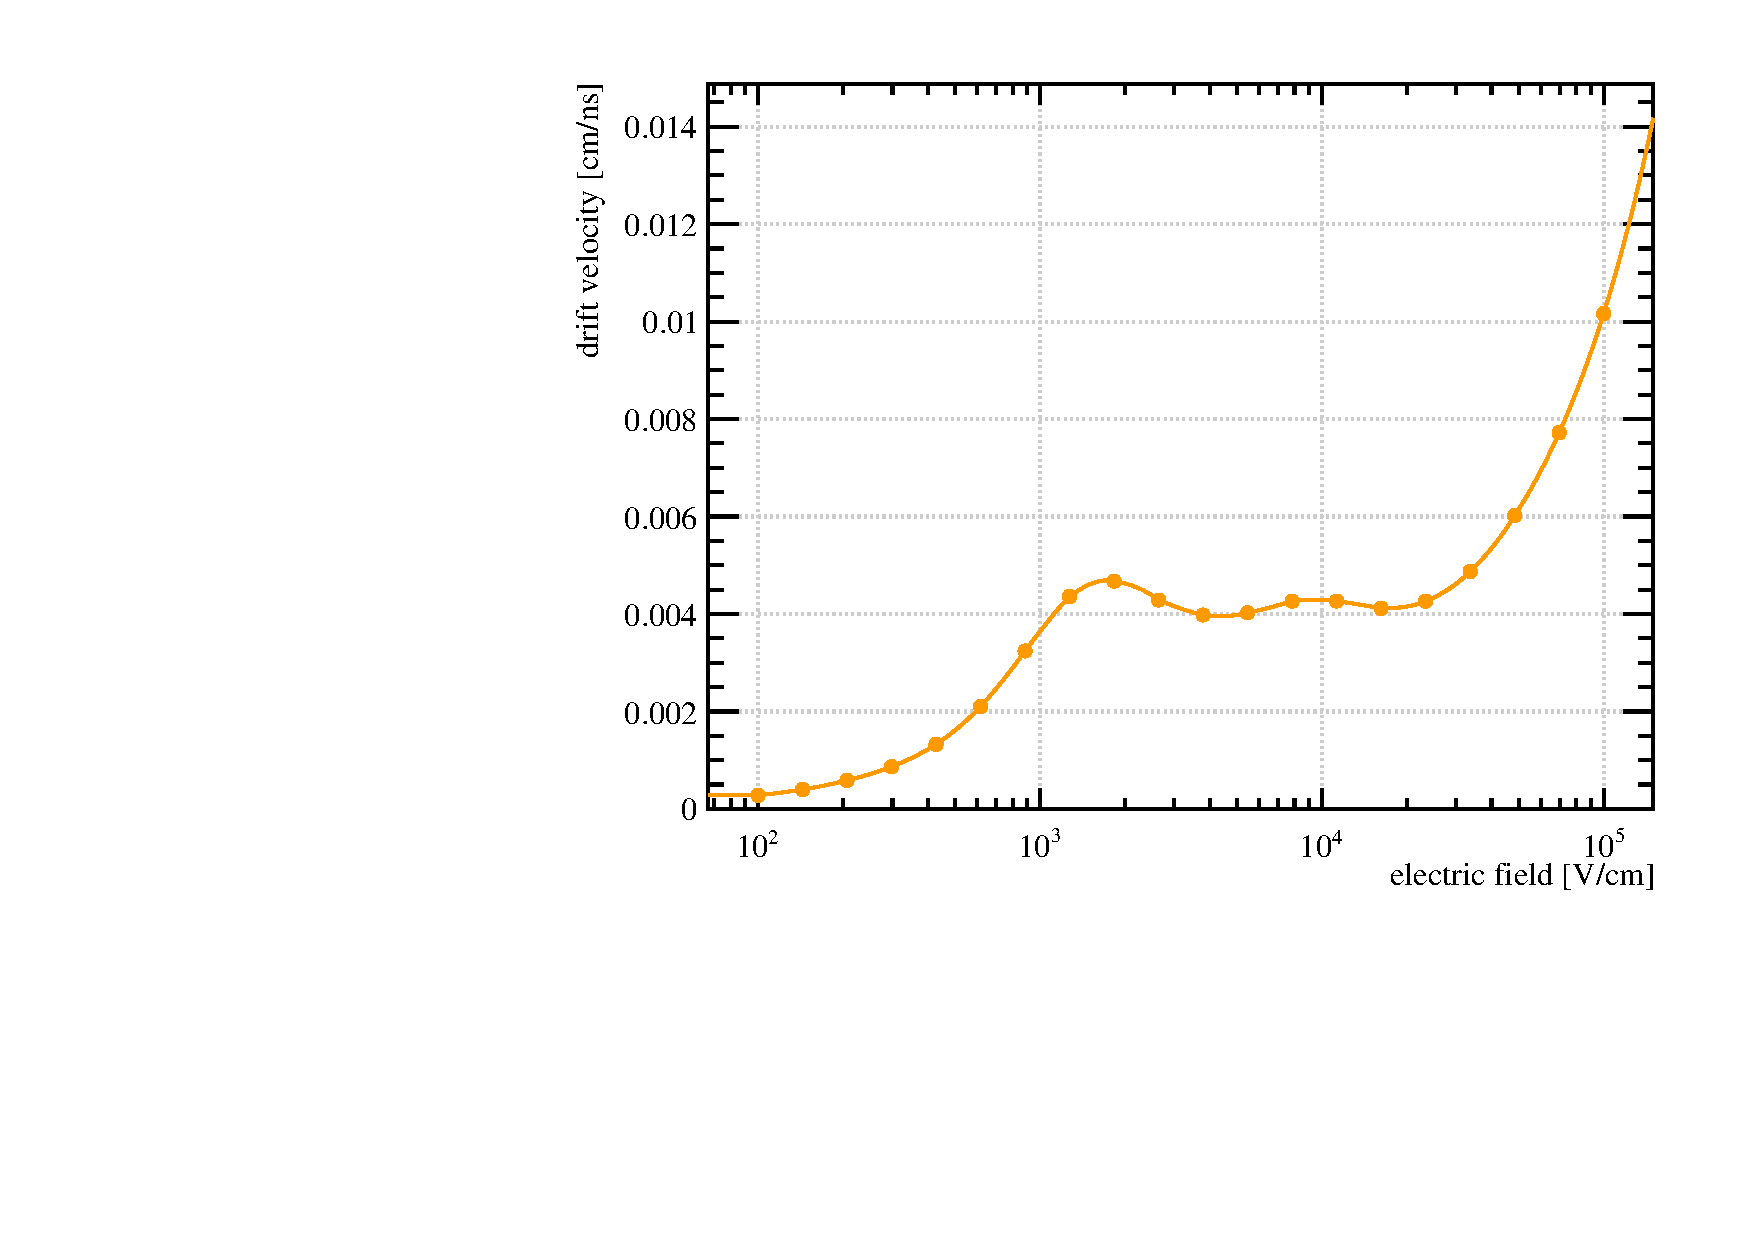
\includegraphics[width=0.6\linewidth]{Chapters/EjemploGarfield/TuboDeriva/build/drift_velocity.pdf}
\end{center}

Ahora podemos calcular el  \textbf{campo eléctrico} que se hace a través de \texttt{ComponentAnalyticField}, que básicamente maneja la disposición de cables, planos y tubos: \\

\begin{lstlisting}[language=C++,style=c++]
ComponentAnalyticField cmp;
\end{lstlisting} 

\vspace*{1em}

Tenemos que introducir el medio que hemos definido en la región activa: \\

\begin{lstlisting}[language=C++,style=c++]
cmp.SetMedium(&gas);
\end{lstlisting} 

\vspace*{1em}

Lo siguiente que tenemos que hacer es añadir los elementos que definen el campo eléctrico, i.e. el cable (denominado ``s'') y el tubo: \\


\begin{lstlisting}[language=C++,style=c++]
// Radio del cable [cm]
const double rWire = 25.e-4;

// Radio del tubo externo [cm]
const double rTube = 0.71;

// Voltajes 
const double vWire = 2730.;
const double vTube =    0.;

// Añadimos el cable en el centro de la disposición 
cmp.Addwire(0,0,2 * rWire, vWire, "s");

// Añadimos el tubo
cmp.AddTube(rTube, vTube, 0);
\end{lstlisting} 
\vspace*{1em}

Finalmente, creamos un \texttt{Sensor}, que es un objeto que actúa como interfaz en la clase transporte  discutido más abajo: \\


\begin{lstlisting}[language=C++,style=c++]
// Calculamos el campo eléctrico usando el objeto Componente cmp.
Sensor sensor(&cmp);
// Hacemos una petición para que calcule la señal del electrodo llamado s
//     usando el campo dado por el objeto Componente cmp.
sensor.AddElectrode(&cmp,"s");
\end{lstlisting} 
\vspace*{1em}

Ahora necesitadmos definir el intervalo temporal en el que la señal es guardada y la granularidad (ancho del bin). Podemos usar 1000 bins con un ancho de 0.5 ns \\

\begin{lstlisting}[language=C++,style=c++]
const double tstep = 0.5;
const double tmin = -0.5 * tstep;
const unsigned int nbins = 1000;
sensor.SetTimeWindow(tmin,tstep,nbins);
\end{lstlisting} 
\vspace*{1em}

Ahora lo que nos queda es \textbf{simular la ionización producida} por la partícula en el tubo de carga usando Heed, de un muón, con por ejemplo, 170 GeV. \textit{Track} significa camino o trayectoria en ingles. \\

\begin{lstlisting}[language=C++,style=c++]
TrackHeed track(&sensor);
track.SetParticle("muon");
track.SetEnergy(170.e9);
\end{lstlisting} 
\vspace*{1em}

Las curvas (lineas) de deriva de los electrones se crean usando el método de integración Runge-Kutta:fehlberg (RKF), implementada en la clase \texttt{DriftLineRKF}. Este método usa las tablas previamente computadas de parámetros de transporte para calcular las líneas de deriva y su multiplicación: \\


\begin{lstlisting}[language=C++,style=c++]
DriftLineRKF drift(&sensor);
\end{lstlisting} 
\vspace*{1em}

Consideremos ahora que la pista pasa a una distancia de 3 mm del centro del hilo. Después de simular el paso de la partícula cargada, nos tenemos que fijar en los ``clusters'' (agrupaciones de partículas cargadas producidas por la partícula primaria) y su movimiento en el dispositivo. Así pues, calculamos las líneas de deriva para cada electrón producido en el cluster: 

\begin{lstlisting}[language=C++,style=c++]
const double rTrack = 0.3;
const double x0=rTrack;
const double y0 = -sqrt(rTube * rTube - rTrack * rTrack)
track.NewTrack(x0,y0,0,0,0,1,0);
// Hacemos un bucle sobre los clusters producidos por el camino (track)
for (const auto& cluster: track.GetClusters()) {
    // Bucle alrededor de los electrones del cluster
    for (const auto& electron: cluster.electrons) {
        drift.DriftElectron(electron.x,electron.y,electron.z,electron.t)
    }
}
\end{lstlisting} 
\vspace*{1em}

Como una comprobación de la simulación podemos visualizar las líneas de deriva. Antes de simular el recorrido de la partícula cargada y las curvas de deriva de los electrones, tenemso que decirle a \texttt{TrackHeed} y \texttt{DriftLineRKF} que pase las coordenadas de los clusters y los puntos de las líenas de deriva al objeto \texttt{ViewDrift}, que se encarga de graficarlas:  \\

\begin{lstlisting}[language=C++,style=c++]
// Creamos un canvas
cD = new TCanvas ("cD"," ", 600, 600);
ViewDrift driftView;
drift.EnablePlotting(&driftView);
track.EnablePlotting(&driftView);
cellView.SetCanvas(cD);
cellView.Plot2d();
constexpr bool twod=true;
constexpr bool drawaxis = false;
driftView.Plot(twod,drawaxis);
cD->SaveAs("drift_view.pdf");
delete cD;
\end{lstlisting} 
\vspace*{1em}
Podemos graficar la señal inducida en el hilo/cable por la deriva de los electrones simulados:  \\

\begin{lstlisting}[language=C++,style=c++]
TCanvas* cS = new TCanvas("cS","",600,600);
sensor.PlotSignal("s",cS);
\end{lstlisting} 
\vspace*{1em}

\begin{center}
    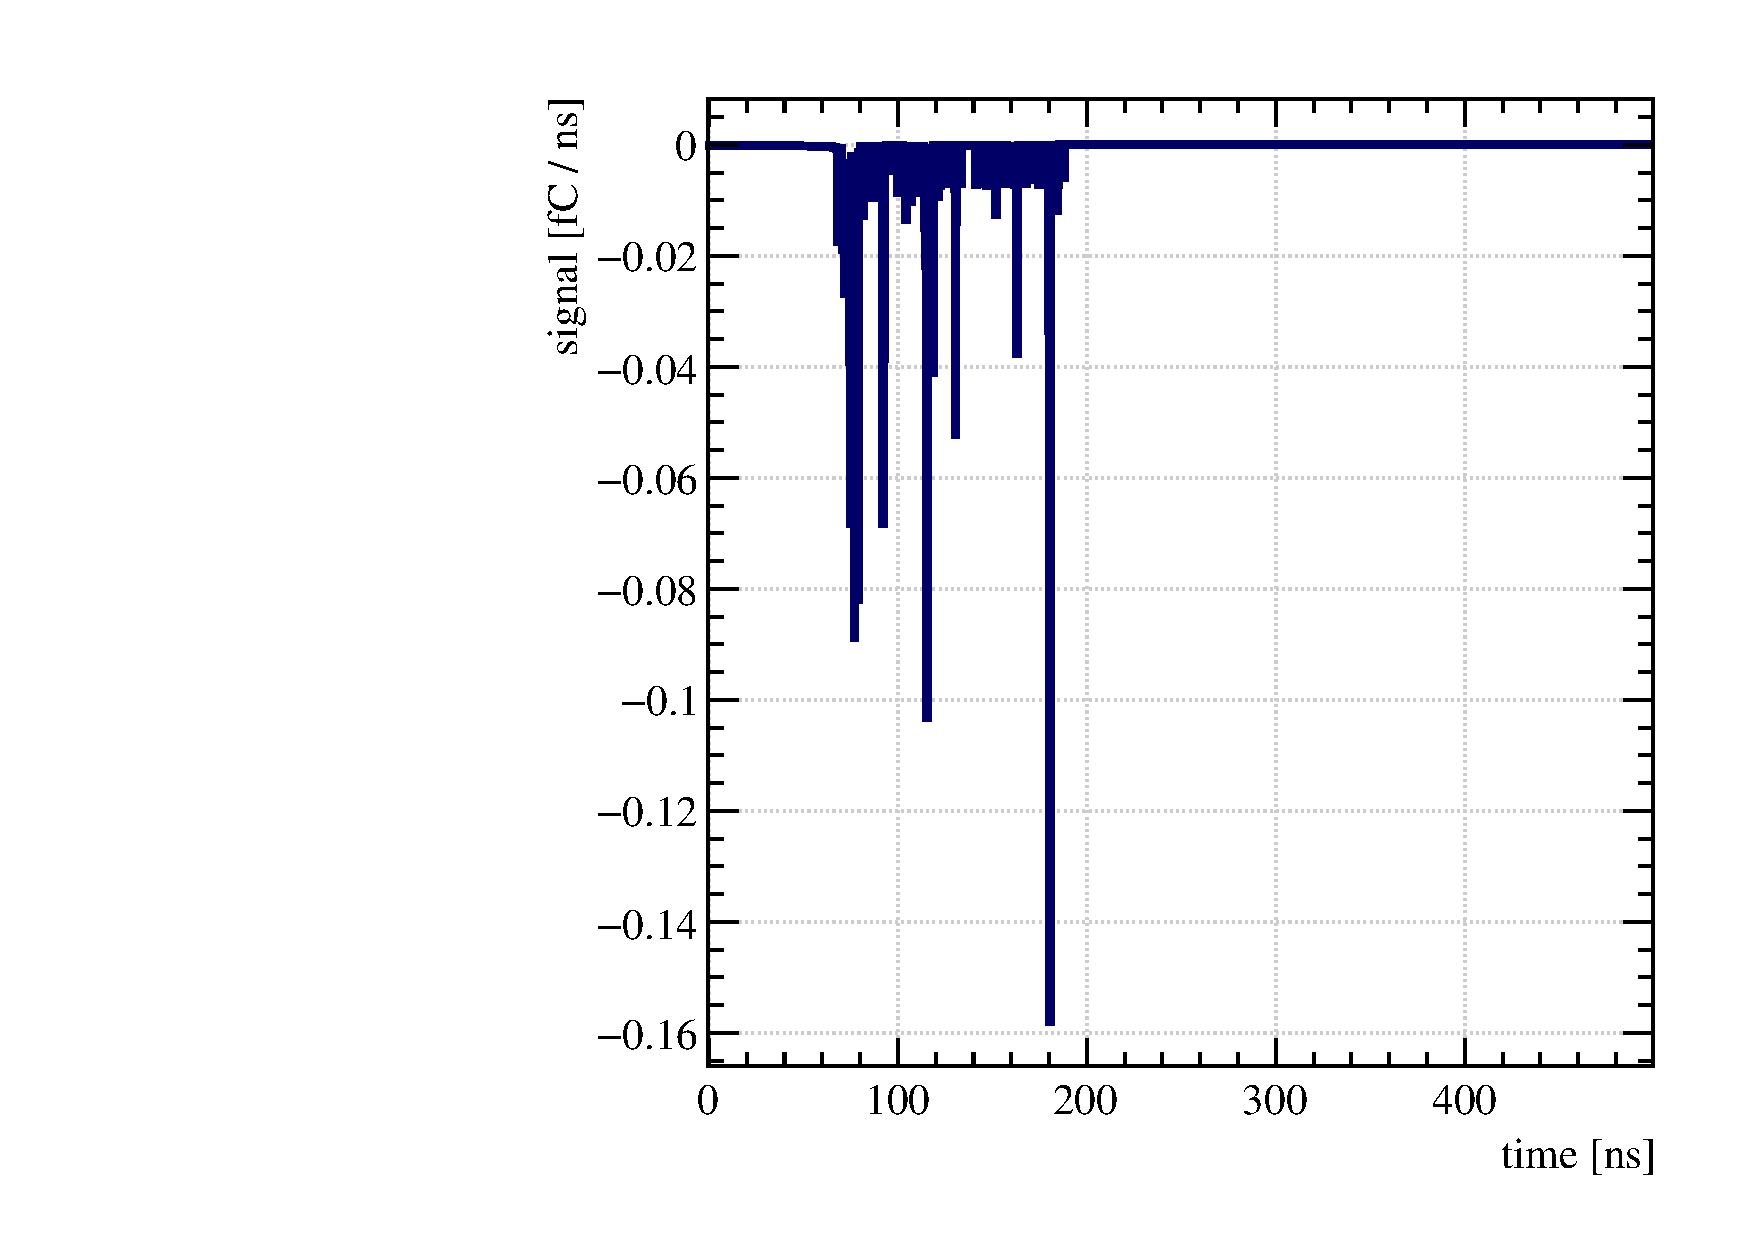
\includegraphics[width=0.6\linewidth]{Chapters/EjemploGarfield/TuboDeriva/build/signal.pdf}
\end{center}

Si quisieramos considerar la contribución de los iones producidos en la avalancha necesitamos importar tablas de mobilidades de iones: \\


\begin{lstlisting}[language=C++,style=c++]
gas.LoadIonMobility("LoadIonMobility_Ar+_Ar.txt")
\end{lstlisting} 
\vspace*{1em}

que, por defecto, \texttt{DriftLineRKF} las incluirá en la simulación. 






\end{Ejemplo}